\documentclass[conference]{IEEEtran}
\IEEEoverridecommandlockouts

\usepackage{amsmath}
\usepackage{booktabs}
\usepackage{graphicx}
\usepackage{array}
\usepackage{url}
\usepackage{xspace}
\usepackage{cite}

\setlength{\textfloatsep}{10pt plus 2pt minus 2pt}
\setlength{\dbltextfloatsep}{12pt plus 2pt minus 2pt}
\setlength{\floatsep}{8pt plus 2pt minus 2pt}
\setlength{\dblfloatsep}{8pt plus 2pt minus 2pt}

\newcommand{\system}{HeteroKV\xspace}
\newcommand{\bzero}{\textsc{B0}\xspace}
\newcommand{\btwo}{\textsc{B2}\xspace}

\title{HeteroKV: Provenance-Tracked Bounded Evidence Packing for Source-Cued Cloud Document QA}

\author{
\IEEEauthorblockN{Haoran An\IEEEauthorrefmark{1}, Qide Mao\IEEEauthorrefmark{1}, and Yuzhong Cao\IEEEauthorrefmark{2}\thanks{Corresponding author: Yuzhong Cao.}}
\IEEEauthorblockA{\IEEEauthorrefmark{1}Beijing City University, Beijing, China\\
Email: ahr123456@bcu.edu.cn; penguinsama8@gmail.com}
\IEEEauthorblockA{\IEEEauthorrefmark{2}Peking University, Beijing, China\\
Email: caoyuzhong@pku.edu.cn}
}

\begin{document}
\maketitle

\begin{abstract}
Document question answering (QA) services often receive a known source handle but must choose how much evidence to activate in a vision-language model (VLM). We present \system, an external evidence-management layer that converts source content into typed, provenance-tracked \emph{MemoryUnits} and constructs budgeted \emph{EvidencePackets}. Its contribution is an inspectable source-scope and payload contract, not a new dominant retrieval algorithm. On an A100 80GB GPU with Qwen2-VL, source-local candidate growth of 5$\times$/3$\times$ changes text-only peak reserved memory by 0.367/0.055 GiB; the one-image path is unchanged. Three endpoint repeats yield identical reserved peaks under this fixed protocol. Fixed-prefix evaluation of 1,000 DocVQA and 2,000 TextVQA questions reaches 0.8742 ANLS under our stated cutoff and 0.7848 local soft VQA, respectively, but uses source-image fallback in 99.9\%/99.1\% of cases. Paired first-500 controls show that text-only packing does not consistently beat OCR-lexical or layout-aware controls; one-image packets instead offer a higher-quality, higher-resource operating point. A real local HTTP vLLM service with preselected packets sustains 26.97 and 6.20 requests/s for these two families at concurrency eight. These are source-cued subset and local-serving results, not official leaderboard scores, unconstrained source discovery, or constant total memory.
\end{abstract}

\begin{IEEEkeywords}
document question answering, multimodal systems, external memory, evidence provenance, bounded inference, vision-language models
\end{IEEEkeywords}

\section{Introduction}
Document QA combines optical character recognition (OCR), layout, and VLM generation. Applications often know the relevant source but still forward excessive content. Large payloads increase accelerator residency and latency; aggressive OCR-only reduction can instead lose visual evidence.

This paper studies the \emph{source/document-cued} setting: each request supplies a source handle, while the system chooses which evidence from that source becomes active. This setting differs from global document retrieval. It is relevant to document workspaces, uploaded-file assistants, and session-bound multimodal agents, where authorization or application state identifies the source but not the answer-bearing region. We therefore ask: \emph{Can a system keep request-scale active evidence bounded as a source-local memory grows, while exposing the quality and resource consequences of different evidence families?}

\system ingests OCR, layout and images as typed \emph{MemoryUnits}, routes by source, ranks source-local units, and emits a budgeted \emph{EvidencePacket} retaining source/transform provenance. \bzero supplies text units without an image; \btwo supplies one bounded source image. They are different payload families, not equal-cost selector alternatives.

The distinction from conventional retrieval-augmented generation (RAG) is operational rather than a replacement retrieval algorithm: source access is explicit, activation limits are checked before invocation, and selected evidence is linked to source transformations. Bounded top-$k$ prompting already exists; our study makes evidence-family cost and fallback behavior observable. The experiments use fixed-prefix subsets, not full-dataset or multi-model evaluations.

Our contributions are:
\begin{itemize}
  \item A source-cued evidence contract linking source scope, transformations, selected units, and activation limits at the VLM boundary.
  \item A reproducible packing pipeline with separate text-only and one-image resource families, recording image fallback rather than attributing its quality to crop selection.
  \item A measured quality--resource study with larger fixed-prefix QA samples, paired selection controls, repeated GPU endpoints, and a shared local serving workload.
\end{itemize}

\section{Related Work}
\textbf{Document and text VQA.} TextVQA tests reading text in natural images~\cite{singh2019textvqa}, and DocVQA tests layout-rich documents~\cite{mathew2021docvqa}. LayoutLM combines text/layout~\cite{xu2020layoutlm}, Donut learns OCR-free understanding~\cite{kim2022donut}, and ColPali retrieves visual document representations~\cite{faysse2025colpali}. We instead study budgeted activation after a source is identified, without a learned visual-retrieval comparison.

\textbf{External retrieval and visual representation.} Retrieval-augmented generation grounds text generation in selected external evidence~\cite{lewis2020rag}. \system likewise separates persistent evidence from active model input, but its evaluated route is source-local and includes OCR/layout features; it does not establish unconstrained semantic source discovery.

\textbf{Efficient inference.} PagedAttention manages shared KV memory~\cite{kwon2023pagedattention}; FlexGen coordinates GPU/CPU/disk placement~\cite{sheng2023flexgen}; H2O and KIVI prioritize/compress KV state~\cite{zhang2023h2o,liu2024kivi}. Our input-side evidence control is complementary. E4 uses vLLM without contributing a scheduling algorithm.

\textbf{Provenance and reproducibility.} Provenance models represent derivations and transformations of data products~\cite{moreau2011provenance}. \system applies this principle to engineering traceability---not as a privacy, integrity, or security guarantee.

Table~\ref{tab:paradigms} compares system layers: full-source prompting retains evidence, text top-$k$ can lose visual relations, and model-internal KV optimization is complementary. \system adds an explicit pre-invocation evidence contract, not a universally stronger ranker.

\begin{table}[!t]
\centering
\caption{Conceptual comparison, not an empirical ranking.}
\label{tab:paradigms}
\scriptsize
\setlength{\tabcolsep}{2.4pt}
\begin{tabular}{p{0.25\columnwidth}p{0.28\columnwidth}p{0.39\columnwidth}}
\toprule
Layer & Active input & Principal boundary \\
\midrule
Full-source VLM & Source text/images & Active payload grows \\
OCR/layout top-$k$ & Ranked text spans & Can lose visual relations \\
Paged/KV methods & Prompted model state & Execution layer, not evidence selection \\
\system \bzero & Typed text units & Capped; no selector dominance \\
\system \btwo & One source image & Capped; different image cost \\
\bottomrule
\end{tabular}
\end{table}

\section{System Model and Design}
\subsection{Scope and invariants}
Let a source $s$ contain external evidence units $U_s=\{u_i\}$. The application supplies $s$ and question $q$. \system constructs a packet $P(q,s)\subseteq U_s$ subject to a fixed budget $\mathcal{B}$:
\begin{equation}
\begin{split}
P(q,s)&=\operatorname{Pack}_{\mathcal{B}}\left(\operatorname{Rank}(q,U_s)\right),\\
|P|_{\mathrm{units/chars/images/pixels}}&\leq\mathcal{B}.
\end{split}
\end{equation}
The configured activation caps are independent of $|U_s|$, but CPU/disk index and ingest cost can grow. Actual tokenizer counts and GPU peaks are measured outputs, not guaranteed constants. The application supplies the source handle; no-source discovery and full-context equivalence are outside the main claim.

\subsection{Typed memory and provenance}
A \emph{MemoryUnit} stores a stable unit identifier, source identifier, modality/type, text or image reference, source-local span or bounding box when available, and transformation metadata (for example, OCR normalization). IDs combine source-local identifiers with SHA-1-derived text/packet keys where applicable; cryptographic security is not claimed. An \emph{EvidencePacket} records the query, source access mode, selected unit identifiers, ranking scores, active token/image counts, prompt payload, and pointers back to the originating units. This design makes every active item traceable to a source record and prevents silent mixing of source-cued and no-source runs.

\begin{figure*}[!t]
\centering
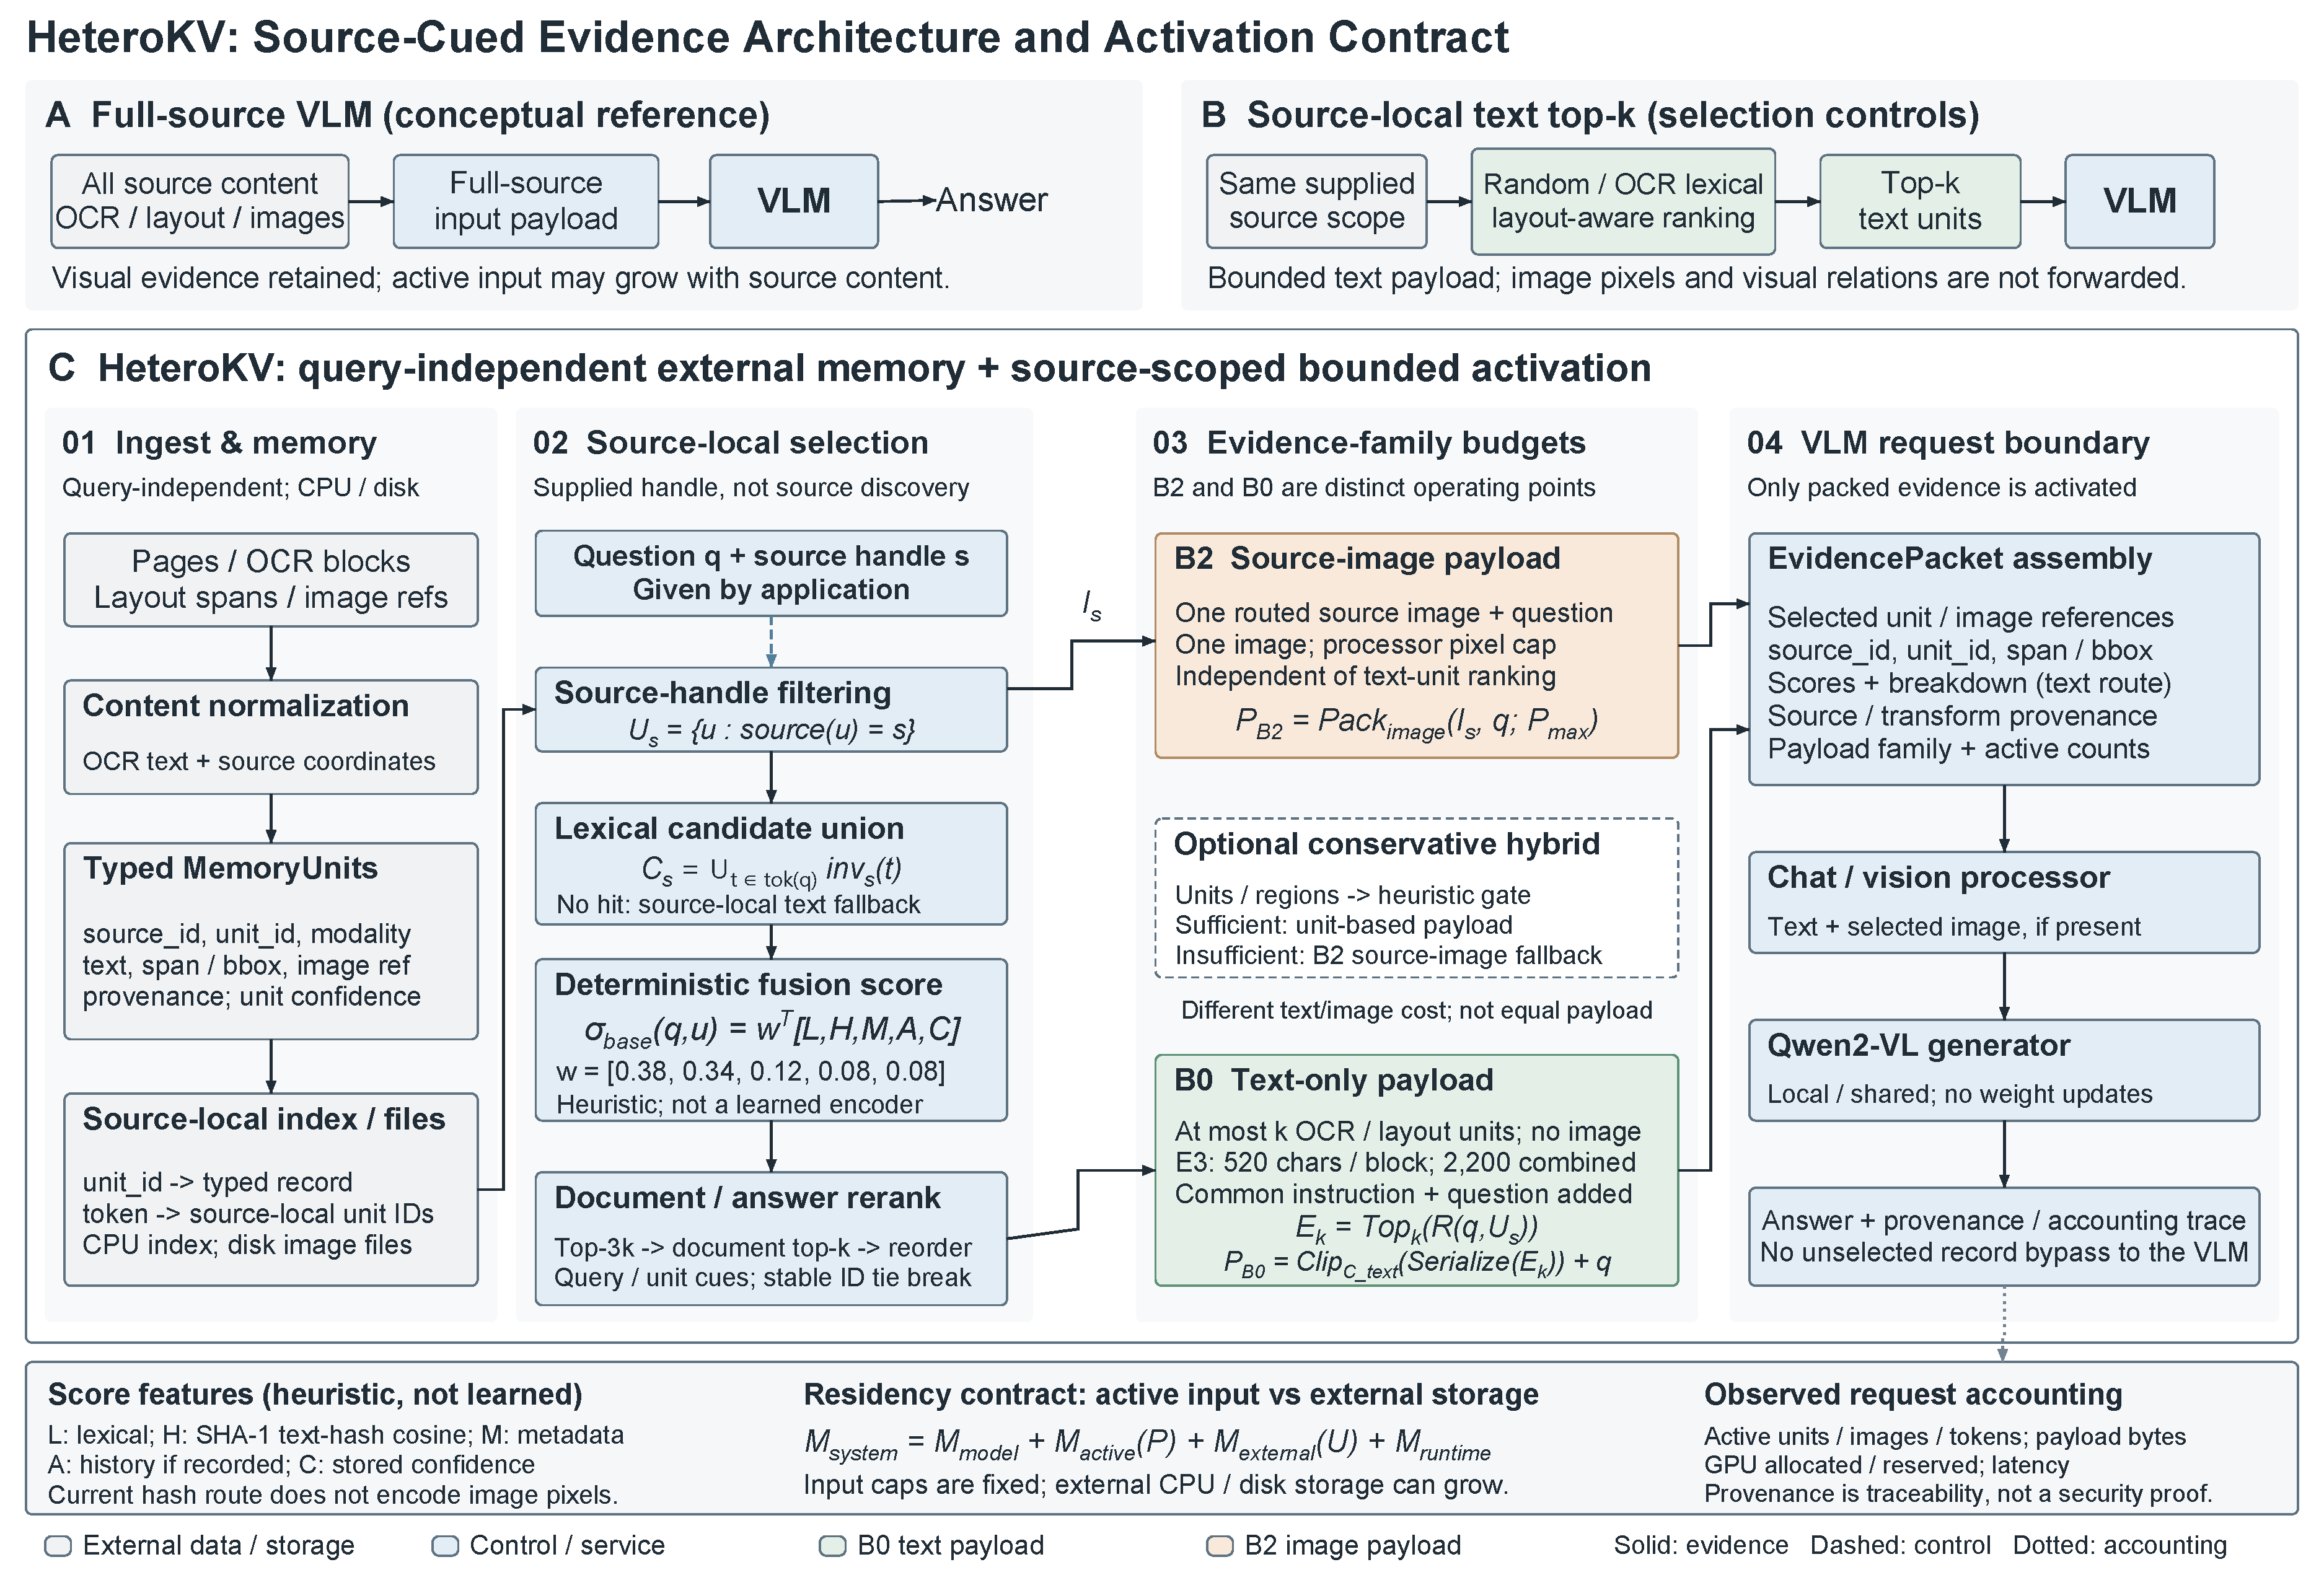
\includegraphics[width=0.98\textwidth,trim=0 35 0 55,clip]{figures/heterokv_architecture_academic.pdf}
\caption{Source-cued architecture and activation contract. A/B are conceptual comparisons. C separates typed ingest, heuristic selection, B0/B2 packing, and generation. B2 bypasses text ranking; the optional hybrid is heuristic. Arrows: solid evidence, dashed control, dotted accounting.}
\label{fig:architecture}
\end{figure*}

\subsection{Ingest, selection, and packing}
Ingest normalizes OCR whitespace, retains layout coordinates when present, and registers page/image records. Query processing follows four steps:
\begin{enumerate}
  \item \textbf{Route}: restrict candidates to the supplied source handle.
  \item \textbf{Score}: compute source-local lexical/OCR and layout-aware features, with deterministic tie handling.
  \item \textbf{Budget}: cap unit count, serialized text, and image count/pixels before invocation.
  \item \textbf{Pack}: serialize selected text and/or one image, record provenance and accounting, then invoke the VLM.
\end{enumerate}
The evaluated ranker is deterministic and heuristic. Its base score is $0.38L+0.34H+0.12M+0.08A+0.08C$, where $L$ is lexical overlap, $H$ is nonnegative cosine similarity of hashed text features, $M$ is metadata match, $A$ is recorded history, and $C$ is unit confidence. The audited hash route uses stable SHA-1 features, not a learned visual or dense encoder. Document and generation rerankers add unit-type and query-cue bonuses, followed by a stable unit-ID tie break. These hand-set weights are not established as optimal by an ablation.

The OCR-lexical control scores each unit as $0.78o+0.12f+0.07c+0.03d$, and the layout control as $0.55o+0.12f+0.20l+0.08c+0.05d$. Here $o$ is the fraction of question terms present, $f$ their normalized frequency, $c/l$ OCR/layout-type indicators, and $d$ a digit indicator. The legacy mode \texttt{bm25\_ocr} lacks inverse-document frequency and BM25 saturation; we therefore call it \emph{OCR lexical}, not standard BM25. Random ordering uses a stable hash of seed, question, and unit ID. Answer labels are not used in scoring.

\begin{figure}[!t]
\centering
\fbox{\begin{minipage}{0.92\columnwidth}
\footnotesize
\textbf{Algorithm 1: Source-cued EvidencePacket construction}\\[-1mm]
\textbf{Input:} question $q$, supplied source handle $s$, source units $U_s$, activation caps $\mathcal{B}$, policy $p$.\\
\textbf{Output:} answer $y$ and accounting/provenance trace $\tau$.\\[0.5mm]
1. Load only the index entries in $U_s$; do not consult answer labels.\\
2. Normalize $q$ and score units with the selected lexical/OCR/layout route.\\
3. Stable-sort; cap units and text, or image count/pixels.\\
4. If $p=\bzero$, pack bounded text units; if $p=\btwo$, pack one source image plus prompt text.\\
5. Emit packet metadata: unit IDs, scores, active counts, payload family, and source/transformation pointers.\\
6. Invoke Qwen2-VL, return $y$, and persist $\tau$ for replay.
\end{minipage}}
\caption{Audited query-time construction. External ingest occurs before this procedure; total CPU/disk storage is not bounded by $\mathcal{B}$.}
\label{alg:packet}
\end{figure}

\subsection{Evidence operating points}
\textbf{\bzero text-only.} The packet uses four units in E1 and up to 12 in E3, without an image. E3 serialization clips each block to 520 characters and the combined evidence text to 2,200 characters, before the common instruction and question. Equal unit caps are not identical token/byte counts; realized input tokens are reported.

\textbf{\btwo bounded source image.} The packet contains one source image plus the shared question/prompt text. This route retains visual evidence and is the current high-quality point. Because image payload and text-unit payload have different representations, \btwo is not treated as an equal-payload comparison against \bzero.

\textbf{Hybrid route.} A heuristic gate decides whether selected units/crops are sufficient, otherwise invoking the source-image route. It is not a trained or calibrated correctness predictor. Image-dominated hybrid quality must not be interpreted as crop-only success.

\subsection{Cost model and policy semantics}
The relevant memory decomposition is
\begin{equation}
M_{\mathrm{system}}=M_{\mathrm{model}}+M_{\mathrm{active}}(P)+M_{\mathrm{external}}(U)+M_{\mathrm{runtime}}.
\end{equation}
The controller caps evidence input, not every byte of $M_{\mathrm{active}}$ or $M_{\mathrm{runtime}}$; kernels and allocators still affect GPU peaks. It does not bound $M_{\mathrm{external}}$, which grows on CPU/disk. We report observed GPU peaks and host-process RSS rather than claim constant total memory.

Likewise, an end-to-end request can be decomposed as $T=T_{\mathrm{route}}+T_{\mathrm{rank}}+T_{\mathrm{pack}}+T_{\mathrm{serve}}$. E3 records ingest and answer time separately. E4 begins after evidence has been selected and therefore measures only the shared service envelope for packed prompts. It cannot be used as an end-to-end retrieval-latency result.

The experiments evaluate fixed operating points, not a learned switch. \bzero favors lower text-input cost; \btwo favors one-image fidelity.

\subsection{Failure behavior and audit trail}
Text-only packets cannot silently acquire an image: fallback is recorded with source access, selected IDs, active counts, payload family, and answer. The controller does not train the VLM. Saved traces do not always retain the full post-clipping prompt, so failure inspection cannot conclusively separate packing loss from generation failure.

\section{Experimental Methodology}
\subsection{Datasets, model, and metrics}
DocVQA~\cite{mathew2021docvqa} uses ANLS in E2 and a \emph{local relaxed QA score} in E1/E3: normalized exact match or a parsed-number match within 5\%. It is not strict exact match. TextVQA~\cite{singh2019textvqa} uses a \emph{local soft VQA score}, $\min(m/3,1)$ for $m$ normalized answer matches; this simplified scorer is not the official leave-one-annotator-out evaluator. Local normalization removes articles/punctuation, without the official number/contraction processing. Results are not directly comparable with leaderboard scores. E3 DocVQA ANLS uses the E2 rule: lowercase, collapse whitespace, and retain edit similarity $\geq0.5$. The checkpoint is local Qwen2-VL-7B; its upstream revision was not recorded. E1/E3 use Transformers 4.57.6, bfloat16, eager attention, at most 1,003,520 image pixels and 24 generated tokens, on an A100 80GB PCIe GPU. PyTorch/CUDA versions were not captured.

\subsection{Four evidence groups}
\textbf{E1---source-local scaling.} Twenty fixed questions per dataset are replayed over increasing candidate-unit prefixes. DocVQA grows from 20 to 100 units (5$\times$); TextVQA grows from 10 to 30 (3$\times$). Endpoint settings are repeated three times. Selection uses stable hashes and no answer labels.

\textbf{E2---larger QA subsets.} The hybrid route is evaluated on the first 1,000 DocVQA and 2,000 TextVQA questions. We recompute scores and 95\% percentile bootstrap intervals with 10,000 resamples (seeds 20260814 and 20260824). These intervals characterize the observed slice, not full-dataset generalization.

\textbf{E3---paired first-500 controls.} Random, OCR lexical, layout-aware, \bzero, and \btwo share identical question/answer prefixes, verified against E2. Text methods share a top-12 unit cap and serialization rule; \btwo uses one image, not equal text payload. Deltas use 10,000 paired bootstrap resamples. Resampling seeds are not multiple GPU experiment seeds. Historical first-100 pilots are excluded from the main control table.

\textbf{E4---shared serving.} A shared Qwen2-VL vLLM 0.18.0 service receives \emph{preselected} E2 packets. Each mode uses 50 DocVQA and 50 TextVQA requests, 10 warm-ups, then 100 measured requests at concurrency 1, 2, 4, and 8, repeated across three fresh services (2,400 measured requests total). The server uses bfloat16, maximum model length 8,192, one image per prompt, prefix caching, chunked prefill, and 0.45 GPU-memory utilization. Client requests specify temperature zero and 24 output tokens; the service logs show a near-greedy model generation configuration. E4 excludes retrieval and index construction. vLLM's internal queue was not exported.

\subsection{Resource-accounting boundary}
E1/E3 report PyTorch peak allocated/reserved memory for the measured process. E4 reports device-level GPU used memory via NVML and server-process RSS. These metrics are not directly interchangeable. E4 observed approximately 34.9--36.1 GiB NVML peaks on an 80GB GPU and is not evidence of operation within 24GB.

\subsection{Artifact integrity and deterministic replay}
We verify immutable source files against their SHA-256 manifest and recompute row-level statistics before paper generation. E1/E3 use stable \texttt{sha1\_v1} feature hashing; legacy process-randomized outputs are excluded. E3 files share identical 500-question signatures and match the E2 prefixes. E4 files contain ten warm-ups and 100 measured requests each. Offline analysis consults saved predictions and labels for metrics only, never to reselect inference evidence.

\section{Results}
\subsection{Bounded active evidence under source-local growth}
Fig.~\ref{fig:e1} reports all E1 points, and Table~\ref{tab:repeat} reports endpoint mean and sample standard deviation (SD). DocVQA text-only reserved peak changes by 0.3672 GiB over 20--100 candidates; TextVQA changes by 0.0547 GiB over 10--30. Image-path reserved peaks are unchanged. Prediction and selected-unit repeat agreement is 1.0. Zero reserved SD describes one deterministic workload and setup, not hardware-independent robustness. This 5$\times$/3$\times$ source-local growth is distinct from historical 50$\times$/100$\times$ external-source-pool observations. All memory values and deltas below are in GiB.

\begin{table}[!t]
\centering
\caption{E1 endpoint means: three repeats, 20 fixed questions. Alloc./Res. are GiB; both SDs are 0.0000. $\Delta$ Res. is relative to each path's smallest candidate setting.}
\label{tab:repeat}
\scriptsize
\setlength{\tabcolsep}{2.2pt}
\begin{tabular}{llrrr}
\toprule
Dataset & Path/units & Alloc. & Res. & $\Delta$ Res. \\
\midrule
Doc & B0/20 & 15.766 & 16.084 & 0.0000 \\
Doc & B0/100 & 15.937 & 16.451 & 0.3672 \\
Doc & B2/20 & 19.371 & 20.285 & 0.0000 \\
Doc & B2/100 & 19.371 & 20.285 & 0.0000 \\
Text & B0/10 & 15.709 & 15.957 & 0.0000 \\
Text & B0/30 & 15.733 & 16.012 & 0.0547 \\
Text & B2/10 & 19.160 & 20.014 & 0.0000 \\
Text & B2/30 & 19.160 & 20.014 & 0.0000 \\
\bottomrule

\end{tabular}
\end{table}

\begin{figure}[!t]
  \centering
  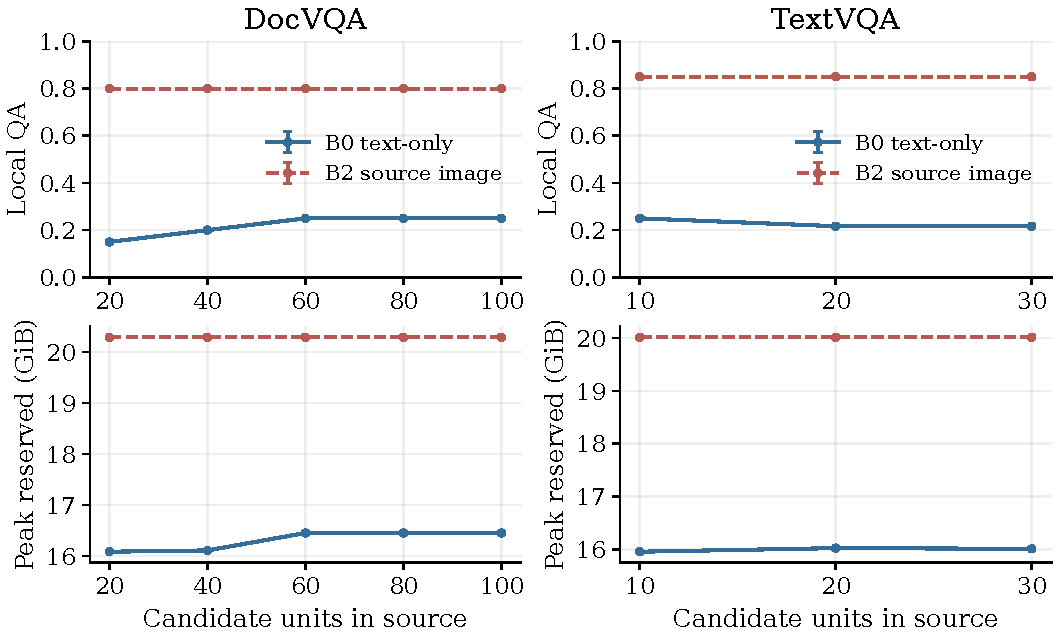
\includegraphics[width=\columnwidth]{figures/e1_source_local_scaling.pdf}
  \caption{E1 source-local candidate growth. Solid and dashed curves are different active payload families. Candidate-unit count changes while the active evidence budget is fixed.}
  \label{fig:e1}
\end{figure}

\subsection{Large-sample quality and fallback behavior}
Table~\ref{tab:e2} summarizes the row-level recomputation. DocVQA reaches 0.8742 ANLS under the stated $\geq0.5$ cutoff and TextVQA reaches 0.7848 local soft VQA, both with 100\% request success. Source-image fallback is invoked in 99.9\% and 99.1\% of cases, respectively. Thus E2 primarily validates the bounded one-image quality route, not a successful crop-only selector.

\begin{table}[!t]
\centering
\caption{E2 image-dominated hybrid quality on fixed-prefix subsets (10,000 resamples). ANLS uses similarity $\geq0.5$; local VQA is simplified, not official leaderboard evaluation.}
\label{tab:e2}
\footnotesize
\setlength{\tabcolsep}{3.5pt}
\begin{tabular}{lrrrc}
\toprule
Dataset & $n$ & Metric & Score & 95\% CI \\
\midrule
DocVQA & 1000 & ANLS & 0.8742 & [0.8543, 0.8930] \\
TextVQA & 2000 & Local VQA & 0.7848 & [0.7673, 0.8015] \\
\bottomrule

\end{tabular}
\end{table}

\subsection{Selection controls and quality--resource tradeoffs}
Fig.~\ref{fig:e3} and Table~\ref{tab:e3} compare E3 operating points. On DocVQA's local relaxed QA, \bzero (0.418) beats random (0.248) but not OCR lexical (0.428) or layout selection (0.452). Strict normalized exact match is instead 0.362 for B0, 0.372 for lexical, 0.386 for layout, and 0.818 for B2. On TextVQA's local soft VQA, \bzero reaches 0.3827 versus 0.3720 and 0.3740; both paired intervals include zero. These results do not establish selector superiority. ANLS recomputation reinforces this limitation (Table~\ref{tab:diagnostic}).

\btwo reaches 0.8400 DocVQA and 0.7893 TextVQA. Its paired improvement over \bzero is +0.422 [0.372, 0.470] and +0.4067 [0.360, 0.453], respectively. It also uses one image and approximately 20.42/20.27 GiB peak reserved memory, whereas unit-text methods use no images and about 16.81--17.09/16.53--16.73 GiB. The result is a quality--resource frontier, not proof that \btwo is a better text selector.

On DocVQA's local relaxed QA, \bzero's advantage over random is +0.170 [0.124, 0.216], while deltas against OCR lexical and layout are $-0.010$ [$-0.042$, 0.022] and $-0.034$ [$-0.068$, 0.000]. On TextVQA's local soft score, lexical/layout deltas are +0.0107 [$-0.0193$, 0.0407] and +0.0087 [$-0.0193$, 0.0360]. Recomputed DocVQA ANLS gives \bzero minus layout $-0.0575$ [$-0.0881$, $-0.0274$] (10,000 paired resamples, seed 20261011). These intervals are not adjusted for multiple comparisons.

\begin{figure}[!t]
  \centering
  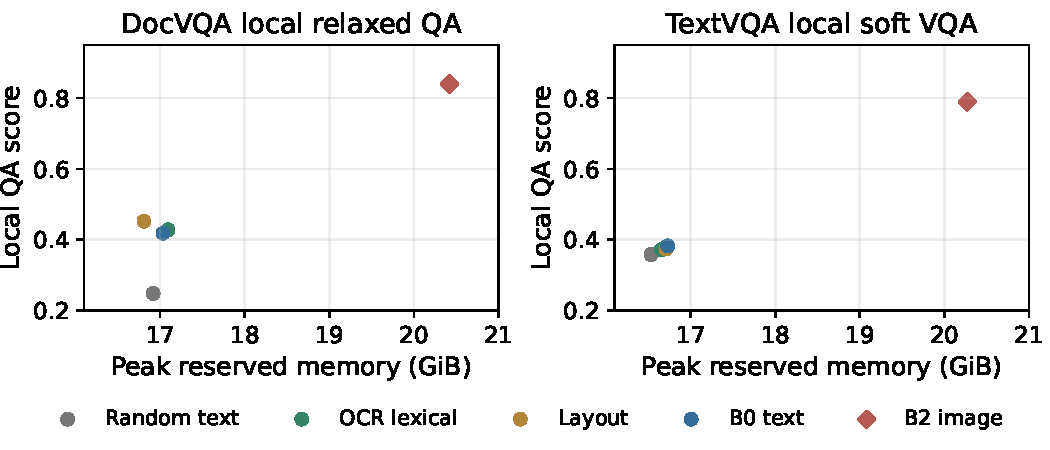
\includegraphics[width=\columnwidth]{figures/e3_quality_resource_pareto.pdf}
\caption{E3 first-500 local QA versus peak reserved memory. DocVQA uses relaxed QA, TextVQA simplified soft VQA, not official leaderboard scores. \btwo is a distinct one-image family; text-unit methods use no image.}
  \label{fig:e3}
\end{figure}

\begin{table*}[!t]
\centering
\caption{E3 paired first-500 controls. DocVQA QA is local normalized-exact or 5\%-numeric match; TextVQA QA is local simplified soft VQA. Tokens/Gen. are measured means; Alloc./Res. are PyTorch peaks, and RSS is host-process peak. Text methods share caps, not identical bytes. B2 is a separate one-image family (1,003,520-pixel cap), not an equal-payload selector.}
\label{tab:e3}
\scriptsize
\setlength{\tabcolsep}{3.2pt}
\begin{tabular}{llrrrrrrr}
\toprule
Dataset & Method & QA & Tokens & Images & Gen. (ms) & Alloc. (GiB) & Res. (GiB) & RSS (GiB) \\
\midrule
Doc & Random text & 0.2480 & 1165.5 & 0 & 306.6 & 16.255 & 16.918 & 5.241 \\
Doc & OCR lexical & 0.4280 & 1052.4 & 0 & 303.1 & 16.294 & 17.094 & 5.239 \\
Doc & Layout & 0.4520 & 1001.6 & 0 & 286.8 & 16.287 & 16.809 & 5.245 \\
Doc & B0 text & 0.4180 & 917.4 & 0 & 281.5 & 16.260 & 17.033 & 5.238 \\
Doc & B2 image & 0.8400 & 1292.1 & 1 & 642.9 & 19.470 & 20.422 & 5.377 \\
\midrule
Text & Random text & 0.3580 & 911.4 & 0 & 216.5 & 16.054 & 16.531 & 5.241 \\
Text & OCR lexical & 0.3720 & 915.2 & 0 & 221.4 & 16.065 & 16.654 & 5.241 \\
Text & Layout & 0.3740 & 899.6 & 0 & 216.4 & 16.142 & 16.709 & 5.241 \\
Text & B0 text & 0.3827 & 644.5 & 0 & 197.2 & 16.090 & 16.729 & 5.242 \\
Text & B2 image & 0.7893 & 1010.7 & 1 & 426.4 & 19.359 & 20.270 & 5.245 \\
\bottomrule

\end{tabular}
\end{table*}

\subsection{Why text and crop reduction remain limited}
Table~\ref{tab:diagnostic} separates answer coverage from QA. Coverage tests normalized answer substrings in selected unit text \emph{before} prompt clipping, with all 500 questions as denominator. It is not post-packing recall or evidence sufficiency; answers are used only in this offline diagnostic. The trace's secondary compact top-$k$ list is not the text-only generation input and is excluded from this analysis. Greater answer-string coverage can coexist with lower QA: a number/name need not retain its field, table row, or visual context. Type/cue bonuses may favor redundant summaries; text clipping may remove relevant context. These are plausible mechanisms, not causal conclusions from an ablation; saved previews cannot reconstruct all post-clipping evidence.

\begin{table}[!t]
\centering
\caption{E3 reduction diagnostic, $n=500$ each. Cov. is pre-packing answer-substring coverage; QA$|$Cov. is mean QA on covered questions. ANLS is recomputed only for DocVQA.}
\label{tab:diagnostic}
\scriptsize
\setlength{\tabcolsep}{2.4pt}
\begin{tabular}{llrrr}
\toprule
Dataset & Method & Cov. & QA$|$Cov. & ANLS \\
\midrule
Doc & OCR lexical & 0.662 & 0.595 & 0.5068 \\
Doc & Layout & 0.666 & 0.634 & 0.5402 \\
Doc & B0 text & 0.672 & 0.571 & 0.4828 \\
Text & OCR lexical & 0.728 & 0.462 & -- \\
Text & Layout & 0.720 & 0.478 & -- \\
Text & B0 text & 0.684 & 0.489 & -- \\
\bottomrule

\end{tabular}
\end{table}

The hybrid gate combines hand-set unit quality, margin, overlap, OCR/layout, crop availability, and numeric cues, with a DocVQA penalty of 0.18 and threshold 0.95. This score is not a calibrated probability. E2 DocVQA logs show 987/1,000 low-score rejections, 12 missing-duration-unit rejections, and only one accepted unit route. TextVQA has 1,973/2,000 low-score rejections, nine duration-unit rejections, and 18 accepted routes. This explains \emph{why the policy falls back}, not whether rejected crops would answer incorrectly. The latter requires paired crop/image generation. Neighbor-preserving crop expansion and a calibrated sufficiency gate remain future experiments.

\subsection{Shared-service concurrency}
Fig.~\ref{fig:e4} shows the E4 serving envelope. From concurrency 1 to 8, \bzero throughput grows from 9.511 to 26.971 requests/s while mean p95 latency grows from 0.246 to 0.752 s. \btwo grows from 3.118 to 6.198 requests/s, with p95 from 1.405 to 3.202 s. All 2,400 measured requests succeed. The observed response-quality aggregates remain stable across concurrency, but the two payload families have different quality and cost.

\begin{table}[!t]
\centering
\caption{E4 local HTTP serving: three fresh services; throughput mean $\pm$ SD, p95 and device-NVML means. NVML SD is 0 except B2 at concurrency 8 (0.214 GiB). Retrieval is excluded.}
\label{tab:e4}
\scriptsize
\setlength{\tabcolsep}{2.2pt}
\begin{tabular}{llrrr}
\toprule
Mode & Conc. & Throughput & p95 (s) & NVML GiB \\
\midrule
B0 & 1 & $9.511\pm0.042$ & 0.246 & 34.864 \\
B0 & 2 & $14.389\pm0.123$ & 0.330 & 34.864 \\
B0 & 4 & $21.069\pm0.057$ & 0.476 & 34.864 \\
B0 & 8 & $26.971\pm0.192$ & 0.752 & 34.864 \\
\midrule
B2 & 1 & $3.118\pm0.041$ & 1.405 & 36.147 \\
B2 & 2 & $4.308\pm0.039$ & 1.492 & 36.147 \\
B2 & 4 & $5.339\pm0.035$ & 2.406 & 35.714 \\
B2 & 8 & $6.198\pm0.031$ & 3.202 & 35.923 \\
\bottomrule

\end{tabular}
\end{table}

\begin{figure}[!t]
  \centering
  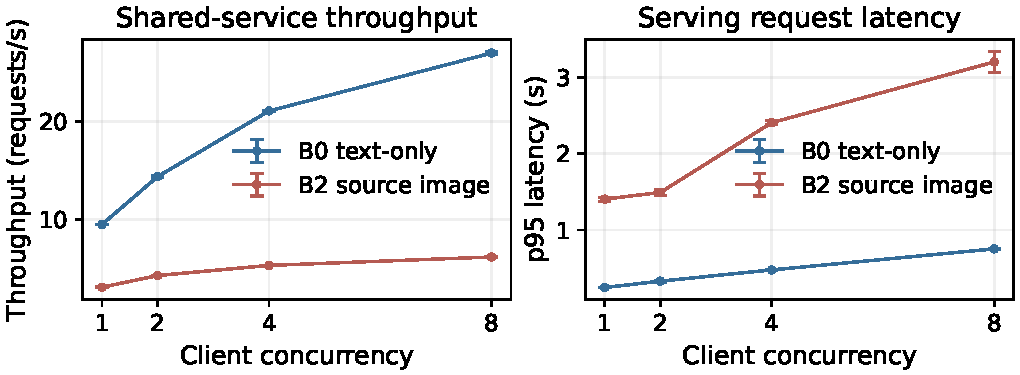
\includegraphics[width=\columnwidth]{figures/e4_shared_serving.pdf}
  \caption{E4 shared vLLM serving with preselected packets. Retrieval and index construction are excluded; error bars show three fresh-service repeats.}
  \label{fig:e4}
\end{figure}

\subsection{Recorded and unmeasured costs}
E3 generation time in Table~\ref{tab:e3} excludes ingest and parts of request preparation. Host RSS of 5.238--5.377 GiB is combined process memory, not isolated index size. The E4 100-request workload carries 155,773 recorded text bytes per family and additionally 32,660,962 image bytes for \btwo. These are workload payloads, not all HTTP framing bytes or billable API tokens, and cannot replace unrecorded E3 per-request bytes. CPU index, disk/cache growth, provenance-logging overhead, isolated routing/packing latency, and provider-side cost remain unmeasured. E1/E3 are actual GPU executions and E4 is a live localhost service, not artifact simulation; neither establishes commercial-cloud or remote-network performance.

\section{Discussion and Limitations}
\textbf{Operational interpretation.} The source-cued contract exposes a workload-dependent choice: \bzero offers smaller inputs and higher service throughput, while \btwo preserves more QA quality at higher image cost. This does not establish a better ranker or improved source discovery.

\textbf{What remains open.} Source discovery is not solved; the application must supply a source handle. Text-only ranking does not consistently beat OCR lexical or layout controls, and the crop/hybrid branch is not main-ready. Standard BM25 and learned visual retrievers such as ColPali remain missing comparisons: hashed features are not a substitute. E1's 5$\times$/3$\times$ growth cannot establish an asymptotic law. E4 excludes retrieval/index construction and exposes no internal queue; its NVML memory is not directly comparable with PyTorch peaks. Checkpoint revision and PyTorch/CUDA versions are missing. Provenance enables engineering audit, not access control, privacy, tamper resistance, or security guarantees.

\textbf{Threats to validity.} E1 uses 20 fixed questions; E2 is image-fallback dominated. E3 uses one checkpoint, one generation seed, and one budget. Local QA scorers are not official leaderboard evaluators; ANLS cutoff ties affect E2 (0.8672 with strict $>0.5$, versus 0.8742 here). Bootstrap intervals are conditional on fixed-prefix sampling, without correction for selection bias or multiple comparisons. Full-dataset and multi-budget/multi-seed robustness are unproven. E4 uses localhost traffic and preselected packets; remote-network variability and multi-tenant interference remain untested.

\section{Conclusion}
\system exposes a source-cued quality--resource tradeoff through typed, traceable, budgeted evidence. Text-only input reduces resource use but does not consistently beat simple controls; one source image preserves more QA quality at higher cost. The results support external evidence management, not superior retrieval or full-context equivalence. Future work requires learned region selection, broader equal-budget controls, and complete end-to-end cost measurement.

\bibliographystyle{IEEEtran}
\bibliography{references}

\end{document}








